%\documentclass[10pt]{article}
\documentclass[10pt]{tufte-handout}


\usepackage[utf8]{inputenc}
\renewcommand*{\familydefault}{\sfdefault}

\usepackage{graphicx}      
\usepackage{hyperref}       
\usepackage{amsmath, amssymb}

%\usepackage{fullpage}

\usepackage{tikz}


\title{A probabilistic user model for information retrieval}
\author{A1, A2}
\date{}

\begin{document}
\maketitle
\begin{abstract}
 A general level probabilistic user model for information retrieval is derived from the basic problem definition. The model is shown to work on various example scenarios and extensions such as new modes of feedback are discussed.
\end{abstract}

\section{Introduction}

What IR is not: recommender systems, 'proactive' (=recommender systems), browsing, 

The continuum from exact item match to exploration of new consepts. Where to draw the line between IR and browsing. Or should such a line be drawn?




\section{Definition}

Definitions in literature, common denominator at a conceptual level.

\subsection{Problem}
An information retrieval system needs to solve the problem of incomplete knowledge of user's information need. Key components must be defined in order to realize any such system.

First component is a known collection $C$ of retrieval items. Each item $i \in C$ in the collection must have a quantification: Call such quantification the feature representation $x_i\in \mathcal X$ with some [metric] space $\mathcal X$. 

For example, a piece of music can be described by the artist, title and record labels, each represented as value 1 of a corresponding binary variable in the joint space of all possible artist, title and record names. 

Second component is the representation of information need. This can be formalized by equating the information need $\theta$ with a distribution in the feature space. For example with some parametric distribution family $p_\theta$ we would set $P(event\ A) = \int_A p_\theta (x) dx$.

Last component is the representation of item relevance, expressed as a scalar variable $r_i\in \mathbb R$. A typical choice interprets low value as 'not relevant' and high value as 'relevant'. The unit interval is common, and even the binary model is used with the downside of e.g. losing 0.5 as 'irrelevant'.

Assume also that the collection is too big or that items are too complicated to simply visualize the entire collection.

\subsection{Solution}
The three components $ \theta, x_i, r_i$ are now connected to make the dependency graph of a solution. Note that the minimal solution graph has at least two edges, as any less would render a component independent of the other two and our problem definition redundant.

\begin{marginfigure}%
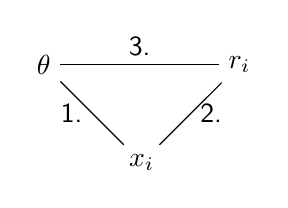
\begin{tikzpicture}[node distance=5em]
  \node[] (doc) {$x_i$};
  \node[above right of=doc] (rel) {$r_i$};
  \node[above left of=doc] (theta) {$\theta$};

  \draw[] (theta) -- node [left] {1.} (doc);
  \draw[] (doc) -- node [right] {2.} (rel);
  \draw[] (theta) -- node [above] {3.} (rel);
\end{tikzpicture}
\caption{Complete graph.}
\label{fig:graph1}
\end{marginfigure}

\begin{marginfigure}%
\begin{tikzpicture}[node distance=5em]
  \node[] (doc) {$x_i$};
  \node[above right of=doc] (rel) {$r_i$};
  \node[above left of=doc] (theta) {$\theta$};

  \draw[] (doc) -- (rel);
  \draw[] (theta) -- (rel);
\end{tikzpicture}
\caption{Solution graph.}
\label{fig:graph2}
\end{marginfigure}

The complete graph (Figure~\ref{fig:graph1}) is not useful: consider
the two possible cases of interaction between $\theta$ and $x_i$. If the user's information need would
affect the feature representation, the change of a user would violate
the first assumption of a fixed collection. Vice versa, the feature
representation should not affect what the user is looking for, but
affect only the system's internal operation. 

The solution has two edges, connecting the information need with the items through
relevance (Figure~\ref{fig:graph2}). The next step is to argue effect direction. Consider the interaction between $\theta$ and $r_i$ (Figure~\ref{fig:graph3}). Natural direction of effect is that infromation need defines what is the relevance of an item. The other direction would imply that the items have some user independent state of relevance, and hence the system would not be providing the user relevant item, but penalize users with non-relevant needs (T: not good... need more thought).

\begin{marginfigure}%
\begin{tikzpicture}[node distance=5em]
  \node (theta) {$\theta$};
  \node[right of=theta] (rel) {$r_i$};
  
  \draw[->] (theta) -- (rel);
\end{tikzpicture}

\noindent\begin{tikzpicture}[node distance=5em]
  \node (theta) {$\theta$};
  \node[right of=theta] (rel) {$r_i$};
  
  \draw[<-] (theta) -- (rel);
\end{tikzpicture}
\caption{Possible effect directions between information need and
  relevance.}
\label{fig:graph3}
\end{marginfigure}

Similarly for $x_i$ and $r_i$ (Figure~\ref{fig:graph4}): if the items are modeled using their relevances then each item would have a different representation when relevances change.

\begin{marginfigure}%
\begin{tikzpicture}[node distance=5em]
  \node (doc) {$x_i$};
  \node[right of=theta] (rel) {$r_i$};
  
  \draw[->] (doc) -- (rel);
\end{tikzpicture}

\noindent\begin{tikzpicture}[node distance=5em]
  \node (doc) {$x_i$};
  \node[right of=doc] (rel) {$r_i$};
  
  \draw[<-] (doc) -- (rel);
\end{tikzpicture}
\caption{Possible effect directions between items and
  relevance.}
\label{fig:graph4}
\end{marginfigure}

The final solution models the relevance variable as a function of information need and fixed item features (Figure~\ref{fig:graph5}). In probabilistic form the model is written as $p(r_i|\theta, x_i)$.

\begin{marginfigure}%
\noindent\begin{tikzpicture}[node distance=5em]
 \node[] (doc) {$x_i$};
  \node[above right of=doc] (rel) {$r_i$};
  \node[above left of=doc] (theta) {$\theta$};

  \draw[->] (doc) -- (rel);
  \draw[->] (theta) -- (rel);
\end{tikzpicture}
\caption{Final solution.}
\label{fig:graph5}
\end{marginfigure}


\section{Properties}

In this section we have interpretation of higher level quantities. Session, information drift, precision-recall, feedback.

\subsection{Definitions of consepts in IR systems}
A session is a bounded and continuous period of system use. Assumption of a constant information need $\theta$ over a session implies constant item relevances and the IR problem is solved by statistical estimation using all data gathered during the session. The problem of session boundary detection is solved by change-point detection in the value of $\theta$. 

Alternative to a fixed $\theta$ is a drifting or shifting information need, reflecting the user's learning or remembering over time. To define a session in such a case requires an extra variable $\Theta$ to represent the larger task involving the information retrieval task. Then $(\theta_t)_{t=1}^T$ is an (autocorrelated) realisation of $\Theta$ over time, i.e. a process approach is needed.

The information need is not possible to be observed in full as this would negate the need for probabilistic retrieval ('retrieve exactly this' is redundant). Querying, item rating and other data collection mechanisms built to the user interface are inprecise and constrained ways for user to give the system some hints of the information need $\theta$. Each mechanism is to be modelled individually as a variable dependent on the information need. For example, query strings and relevance feedback clicks on ranked items are both stochastic expressions originating from the same underlying $\theta$.

To minimize the user's burden of providing hints other sources of data are often used. The user's previous sessions can be used, with some weighting scheme to account for information need jumps and shifts between sessions.

Profiles can be build using some classification rules on user's previous session data. The idea is to build a set of hypothetical states $\theta^1, ..., \theta^ms$ in which the user is assumed to be (i.e. reduction of the information need space). In the running session the IR problem is reduced to mixture distribution weight estimation.

Another technique is to borrow data from the records of other users. The system is build on some balance between the population and the individual's information needs. The population homogeneity assumption holds in some applications, e.g. "each person wants high pagerank web search results" is often a valid assumption, but $\theta$ values can be more heterogeneous for any given set of hints in highly personalized applications such as scientific document database retrievals where the users' tasks vary considerably.

Evaluation of the retrieval: precision-recall, diversity, etc.

The conditional nature of the solution: User's information need given the feature space and collection. Does it match the problem.

\subsection{Latent variable models and Bayesian inference}

The Bayesian approach, the idea of prior knowledge and how profiling etc. are naturally covered.

Borrowing data and the informativeness of a prior.

(T: should the previous subsection descriptions of consepts be here, so the Baysian way could be easily incorporated? Would avoid repetition.)


\section{Examples}

\section{Discussion}


\end{document}  
